\section{Verwandte Themen und Arbeiten}\label{similar_topics}

\subsection{Openbadge}\label{openbadge}

Auf unserem Bildungsweg werden das Erlangen von Fertigkeiten und Kenntnissen mit Zeugnissen und Abschlüssen belegt. Doch oftmals genügt die formale Ausbildung nicht oder hat aufgrund der sich schnell verändernden Technologien oder Kompetenzen nur eine begrenzte Gültigkeit.  
Die Europäische Union fordert eine stärkere Anerkennung von informalem Lernen, damit auch Fertigkeiten und Kenntnisse die ohne ein formales Abschlusszertifikat erworben wurden Anerkennung finden.\cite{Dorn2014}

Doch wie können Personen alle Ihre Fertigkeiten, welche an einer Hochschule, in einer staatlich Anerkannten Ausbildung oder  in einem Online Seminar, in einem Workshop etc. erworben wurden präsentieren, damit auch Arbeitgeber und Bildungsinstitute in der Lage sind, sicherzustellen, dass Bewerber die nötigen Fertigkeiten mitbringen.\cite{alliance_for_excellent_education}

In der digitalen Welt können sogenannte Badges ein Lösungsansatz sein. Ein digitaler Badge ist ein digitales Zertifikat für eine erbrachte Leistung oder eine Fähigkeit. 
Die Mozilla Foundation hat in Zusammenarbeit mit der MacArthur Foundation den Open Badge(OB) Standard entwickelt. Er stellt sicher, dass Alle Badges Informationen über Kriterien und Nachweise erhalten. Die Informationen in einem Badge können auch auf ein Kompetenzframework verweisen, und validiert werden.\cite[4]{alliance_for_excellent_education}

\vspace{1em}

Badges können von Institutionen, Schulen und Arbeitgebern verliehen werden. Sie definieren ein Set von Kompetenzen oder einen Lehrplan und eine Bewertung um festzustellen ob ein Empfänger die notwendigen Anforderungen erfüllt hat. Darüber hinaus können Badges von ihrem "issuer" mit einer verschlüsselten Zusicherung versehen werden, welche bestätigt, dass der "earner" des Badges die geforderte Leistung auch erbracht hat. 
Die Zusicherung kann dann in den Quellcode eines SVG oder PNG Bildes geschrieben werden, sodass dritte später eine elektronisch Überprüfung beim Herausgeber beantragen können. Über das Alignment-Attribut kann ein Badge auch auf eine Quelle verweisen, welche die Kompetenz oder Fähigkeit beschreibt.

\vspace{1em}

\subsection{InLoc}\label{inloc}

Das Europäische Projekt InLOC(Integrating Learning Outcomes and Competences) erlaubt es Kompetenzen und Lernergebnisse verschiedener Kompetenzrahmen in einem einheitlichen semantischen Format abzubilden.

\todo{Wichtig? Mehr Informationen ausarbeiten}

\subsection{ESCO}

In der EU gibt es nach einer Aktuellen Eurostat Statistik ca. 19 Millionen Menschen ohne Beschäftigung. Jedoch haben einige Branchen in Deutschland Probleme Stellen mit qualifiziertem Personal zu besetzen. So blieben im Jahr 2016 In der IT und Telekommunikationsbranche 375.034 Stellen unbesetzt.\cite{Statista2016}
 
Die Europäische Kommission hat dieses Problem erkannt und mit ESCO eine mehrsprachige Klassifizierung für europäische Fähigkeiten, Kompetenzen, Qualifikationen und Berufe entwickelt, deren Zusammenhang durch Berufsprofile verdeutlicht wird.
 
Ein der Aufgaben von ESCO ist es, Die Lücken zwischen dem Arbeitsmarkt und den verschiedenen Bildungssystemen der einzelnen Mitgliedstaaten zu schließen. So unterscheiden sich Qualifikationen welche Menschen in ihren Heimatländern erhalten nicht nur voneinander, sondern können auch oftmals nicht mit aktuellen Entwicklungen des Arbeitsmarktes und dessen Anforderungen mithalten.
\subsection{GraphGist: Competency Management}\label{graphgist}
\subsection{GraphGist: Recommendation System Sandbox}\label{recommender}

Neo4J bietet über die Sandbox eine interaktive Möglichkeit auf einer temporär generierten Instanz im Browser zu arbeiten. Mit Schritt-für-Schritt Anleitungen werden Themen wie "Netzwerk Management" oder die "Panama Papers" in Neo4j näher gebracht. 

Ein für diese Arbeit relevantes Themenfeld bietet die Sandbox "Recommendations".\cite{neo4j} Als Datenquelle für die Instanz stehen die "Open Movie Database"\cite{omdb}, und das MovieLens Projekt\cite{grouplens_2016} zur Verfügung.
Neben einer Erläuterung zum Property Graph Model und einer Einführung in die Cypher Query Language gibt es Beispiele zu verschiedenen Methoden und Metriken für das Filtern von Ergebnissen. Dabei werden verschiedene Ansätze zu den Methoden Inhaltsbasierte Filterung und Kollaborative Filterung erläutert. Ein Beispiel für eine Metrik zum finden von Ähnlichkeiten ist der Jaccard Index. Er ist genau dann 1, wenn zwei Mengen identisch sind. Je weniger Gemeinsame Elemente zwei Mengen besitzen, desto kleiner wird der Jaccard Index und wird 0, wenn keine Gemeinsamkeiten vorliegen.
\begin{center}
	$ J(A,B)=\frac{\mid A\bigcap B\mid }{ \mid A \bigcup B \mid }$

\end{center}

\subsection{RDF Import Neo4J}

Jesús Barrasa ist  \textit{Senior Graph Solutions Consultant at Neo Technology} bei Neo4j, und hat ein Plugin für Neo4j entworfen, mit dessen Hilfe sich RDF Dokumente in Neo4j importieren lassen. So lässt sich mit dem Befehl :
\vspace{1em}

\begin{lstlisting}[frame=htrbl, caption={Das Listing zeigt einen Funktionsaufruf über die Neo4j}, label={lst:result2}]
CALL semantics.importRDF("file:////..../esco_skos.rdf","RDF/XML",
 { languageFilter: 'de', commitSize: 5000 , nodeCacheSize: 250000})	
\end{lstlisting}

Der komplette RDF Graph des ESCO Kataloges mit allen Beziehungen laden und Abfragen.

%\begin{figure}[htb]
% \centering
% 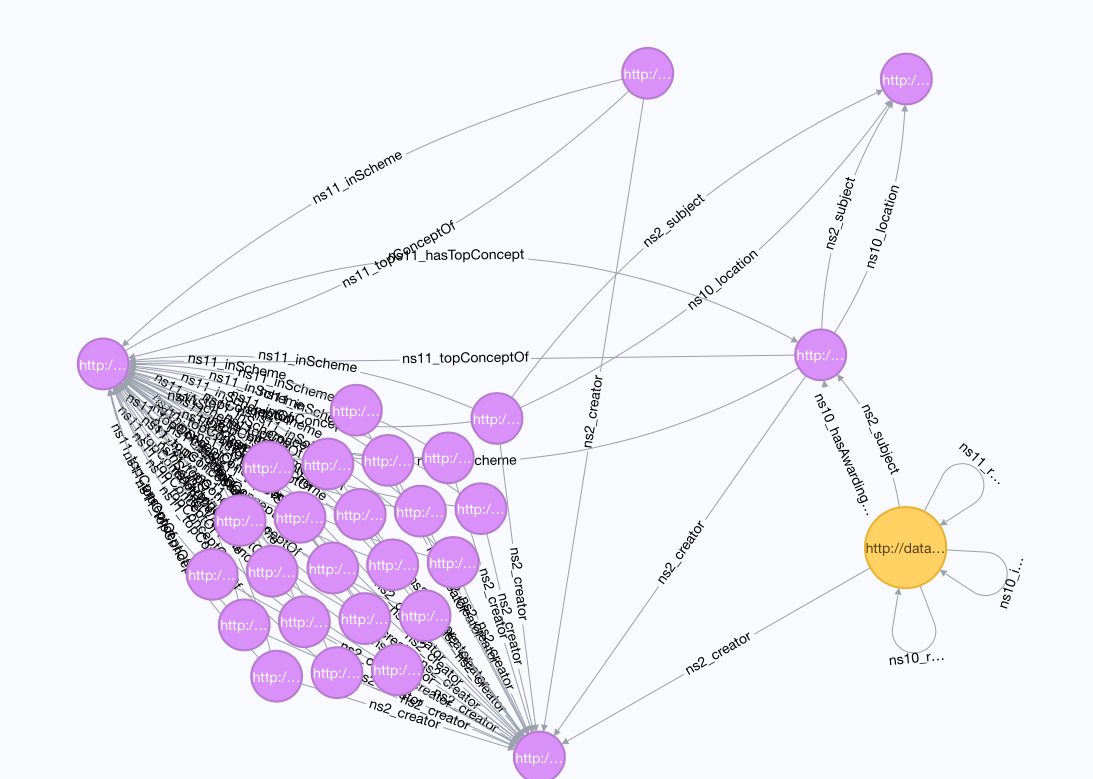
\includegraphics[width=0.3\textwidth,angle=0]{abb/rdf_import_neo4j}
% \caption[Beschreibung]{Beschreibung}
%\label{fig:Beschreibung}
%\end{figure}




